We use an MPC controller with a quadratic and a linear cost for comparison.
The finite RHC approach involves optimizing a cost function subject to the dynamics of the system and the constraints, over a finite horizon of time \cite{Mayne2000}. After an optimal sequence of control inputs is computed, the first input is applied, then at the next step the optimization is solved again.

%\begin{figure}
%\centering
%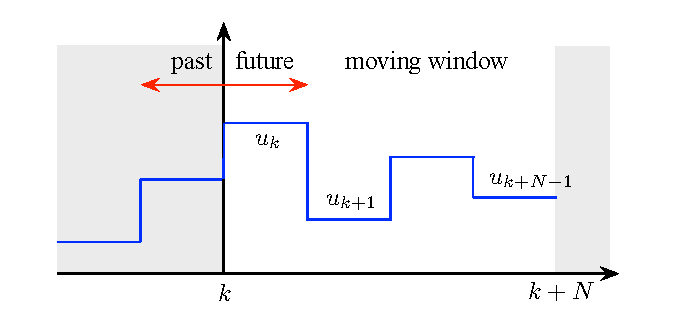
\includegraphics[scale=0.8]{figures/mpc_horizon.eps}
%\caption{Finite-horizon moving window of MPC: at time $k$, the MPC optimization problem is solved for a finite length window of $N$ steps and the first control input $u_k$ is applied; the window then recedes one step forward and the process is repeated at time $k+1$.}
%\captionsetup{justification=centering}
%\label{F:mpc}
%\end{figure}

The objective of the controller is to minimize the energy usage $c^\top u$ while maintaining a desired level of thermal comfort $x_{ref}$ (or $\tT_\mathrm{ref}$).
Therefore, at time step $k$, we solve a continuously linearized MPC problem to determine the optimal sequence of inputs $u^*_{k},\dots,u^*_{k+N-1}$:

\begin{subequations}
	\begin{align}
		& \underset{u_{k+j-1},\epsilon_j}{\text{minimize}} & & \sum_{j=1}^{N+1} ({x}_{k+j} - x_{ref})^\top Q ({x}_{k+j} - x_{ref}) + c^\top u_{k+j-1} +  \lambda\epsilon_j                                                                                                                          \\
		& \text{subject to }                               & & x_{k+j} = Ax_{k+j-1} + B u_{k+j-1} + B_d d_{k+j-1}\label{SE:mpc1}                   \\
		&                                                  & & B       = B_u + B_{xu}[x_{k}] + B_{du}[d_{k+j-1}] \label{SE:mpc2}                   \\
		&                                                  & & \underline{u} \leq u_{k+j-1} \leq \bar{u}                                           \\
		&                                                  & & \underline{x} - \epsilon_j \leq x_{k+j} \leq \bar{x} + \epsilon_j                   \\
		&                                                  & & x_k = x(k)                                                                          \\
		&                                                  & & \epsilon_j \geq 0, \ j = 1,\dots,N+1,            									                 
	\end{align}\label{E:mpc}
\end{subequations} 

\noindent where $Q \in \R^{12 \times 12}$ has all zeros except at $Q^{(1,1)}$ corresponding to the zone temperature, $c \in \R^{4}$ is proportional to cost of using each actuator and $\lambda$ penalizes the slack variables.